\documentclass[11pt,a4paper]{article}
\usepackage{diagbox}
\usepackage{wrapfig}
\usepackage[utf8]{inputenc}
%\usepackage[swedish]{babel}
\usepackage{graphicx}
\usepackage{amsmath}
\usepackage{amssymb}
\usepackage{units}
\usepackage{ae}
\usepackage{icomma}
\usepackage{color}
\usepackage{graphics}
\usepackage{bbm}
\usepackage{float}

\usepackage{caption}
\usepackage{subcaption}

\usepackage{hyperref}
\usepackage{epstopdf}
\usepackage{epsfig}
\usepackage{braket}
\usepackage{pdfpages}
\usepackage{tcolorbox}

\usepackage{svg}
\usepackage{physics}
% \usepackage{tikz}
% \usepackage{pgfplots}
% \pgfplotsset{compat=newest}
% \usepgfplotslibrary{groupplots}
% \usepgfplotslibrary{dateplot}

\newcommand{\N}{\ensuremath{\mathbbm{N}}}
\newcommand{\Z}{\ensuremath{\mathbbm{Z}}}
\newcommand{\Q}{\ensuremath{\mathbbm{Q}}}
\newcommand{\R}{\ensuremath{\mathbbm{R}}}
\newcommand{\C}{\ensuremath{\mathbbm{C}}}
\newcommand{\id}{\ensuremath{\,\mathrm{d}}}
\newcommand{\rd}{\ensuremath{\mathrm{d}}}
\newcommand{\Ordo}{\ensuremath{\mathcal{O}}}% Stora Ordo
\renewcommand{\L}{\ensuremath{\mathcal{L}}}% Stora Ordo
\newcommand{\sub}[1]{\ensuremath{_{\text{#1}}}}
\newcommand{\ddx}[1]{\ensuremath{ \frac{\partial}{\partial #1} }}
\newcommand{\ddxx}[2]{\ensuremath{ \frac{\partial^2}{\partial #1 \partial #2} }}
%\newcommand{\sup}[1]{\ensuremath{^{\text{#1}}}}
\newcommand*\diff{\mathop{}\!\mathrm{d}}
\renewcommand{\vec}[1]{\boldsymbol{\mathbf{#1}}}
\renewcommand{\b}[1]{\ensuremath{ {\bf #1 } }}
\renewcommand{\arraystretch}{1.5}

\title{Effect of toroidicity on runaway generation\\\vspace{.3cm} \large{project course FUF060 in plasma physics}}
\author{Peter Halldestam}
\date{\today}

\begin{document}

\maketitle

\section{Parametrisation of the toroidal magnetic field in}
In \textsc{DREAM}, the shape of the magnetic field is characterised by the elongation $\kappa(r)$, triangularity $\delta(r)$ and Shafranov shift $\Delta(r)$ as illustrated in fig.\ \ref{fig:toroidicity}.
Firstly, the elongation $\kappa$ is a scale factor determining the height of a flux surface in relation to the minor radius coordinate $r\in[0, a]$.
The triangularity $\delta$ determines the horizontal shift of the top-most point of the flux surface and finally, the Shafranov shift $\Delta$, which is the shift from the magnetic axis of the center of a flux surface.
These are set to be linear in $r$ such that they vanish at $r=0$ and is equal to some set value at $r=a$, ie.\ $\kappa(a)=\kappa_a$ and so on.
For instance, the configuration $(\kappa_a, \delta_a, \Delta_a)=(1, 0, 0)$ would yield a circular cross section with concentric flux surfaces.

\begin{figure}[H]
  \begin{minipage}[l]{0.6\textwidth}
    \includesvg[scale=.55]{figs/toroidicity}
  \end{minipage}
  \hfill
  \begin{minipage}[c]{0.4\textwidth}
      \caption{\textit{Tokamak cross section illustrating the three shaping parameters used to define the shape of the magnetic field: elongation $\kappa$, triangularity $\delta$ and Shafranov shift $\Delta$.
      This image is taken from \cite{DREAM}.}}
      \label{fig:toroidicity}
  \end{minipage}
\end{figure}

\noindent
Any position $\vec{x}$ is parametrized with the coordinates $(r, \theta)$ by defining $\vec{x}=R\vec{\hat{R}}+z\vec{\hat{z}}$, where
\begin{align*}
    R
    &=R_0+\Delta(r)+r\cos\{\theta+\delta(r)\sin\theta\},\\
    z
    &=r\kappa(r)\sin\theta.
\end{align*}
With this parametrisation we assume that any flux surface can be characterised by $r$ along with the major radius of the magnetic axis $R_0$ and the three shaping parameters.
This lets us express an arbitrary magnetic field with
\begin{align}
    \label{eq:magnetic}
    \vec{B}(r, \theta)
    =G(r)\grad{\varphi}+\frac{1}{2\pi}\grad{\varphi}\cross\grad{\psi(r)},
\end{align}
where $\varphi$ denotes the toroidal angle, $G(r)$ describes the toroidal magnetic field and finally $\psi(r)$ is the poloidal magnetic flux.
The latter two are set in accordance to an example in \cite{DREAM} (REFERERA BÄTTRE)
\begin{align*}
    G(r)
    &= B_0 R_0\\
    \psi(r)
    &=-\mu_0 I_\text{ref} \bigg[1-\bigg(\frac{r}{a}\bigg)^2\bigg] a
\end{align*}

\section{Runaway generation}
An electron is called runaway if it has reached a speed higher than a critical speed $v_c$ above which the electric field becomes so strong that the accelerating electric force dominates any frictional forces.
The rate at which runaway population grows is given by
\begin{align*}
    \dv{n_\text{re}}{t}
    =\gamma+n_\text{re}\Gamma,
\end{align*}
where $\gamma$ is the runaway rate due to \textit{Dreicer generation} and the second term $n_\text{re}\Gamma$ to \textit{Avalanche generation}.(SKRIV MER OM DESSA)\\

In the following sections, we investigate the effect the three shaping parameters have on the electron runaway generation individually.
\\

\subsection{Dependence on elongation}
\begin{figure}[H]
    \centering
    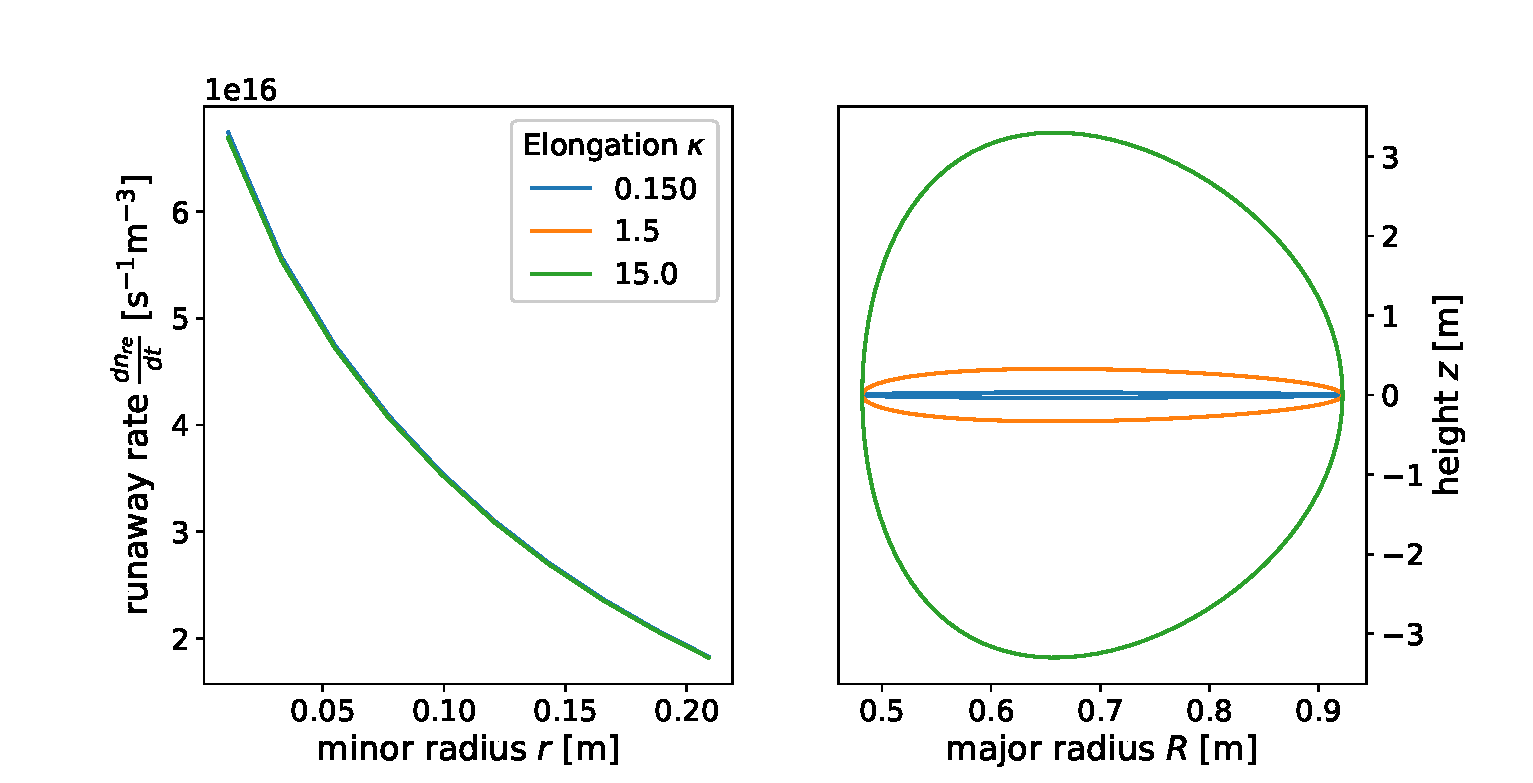
\includegraphics[width=\textwidth]{figs/elongation.eps}
    \caption{\textit{Flux surface averaged electron runaway rate $\langle\diff{n}_{re}/\diff{t}\rangle$ vs.\ minor radius coordinate $r$ for three different elongations $kappa$ (left), and corresponding tokamak cross sections (right).
    No significant effect of $\kappa$ on the runaway rate is observed.}}
    \label{fig:elongation}
\end{figure}

\subsection{Dependence on triangularity}
\begin{figure}[H]
    \centering
    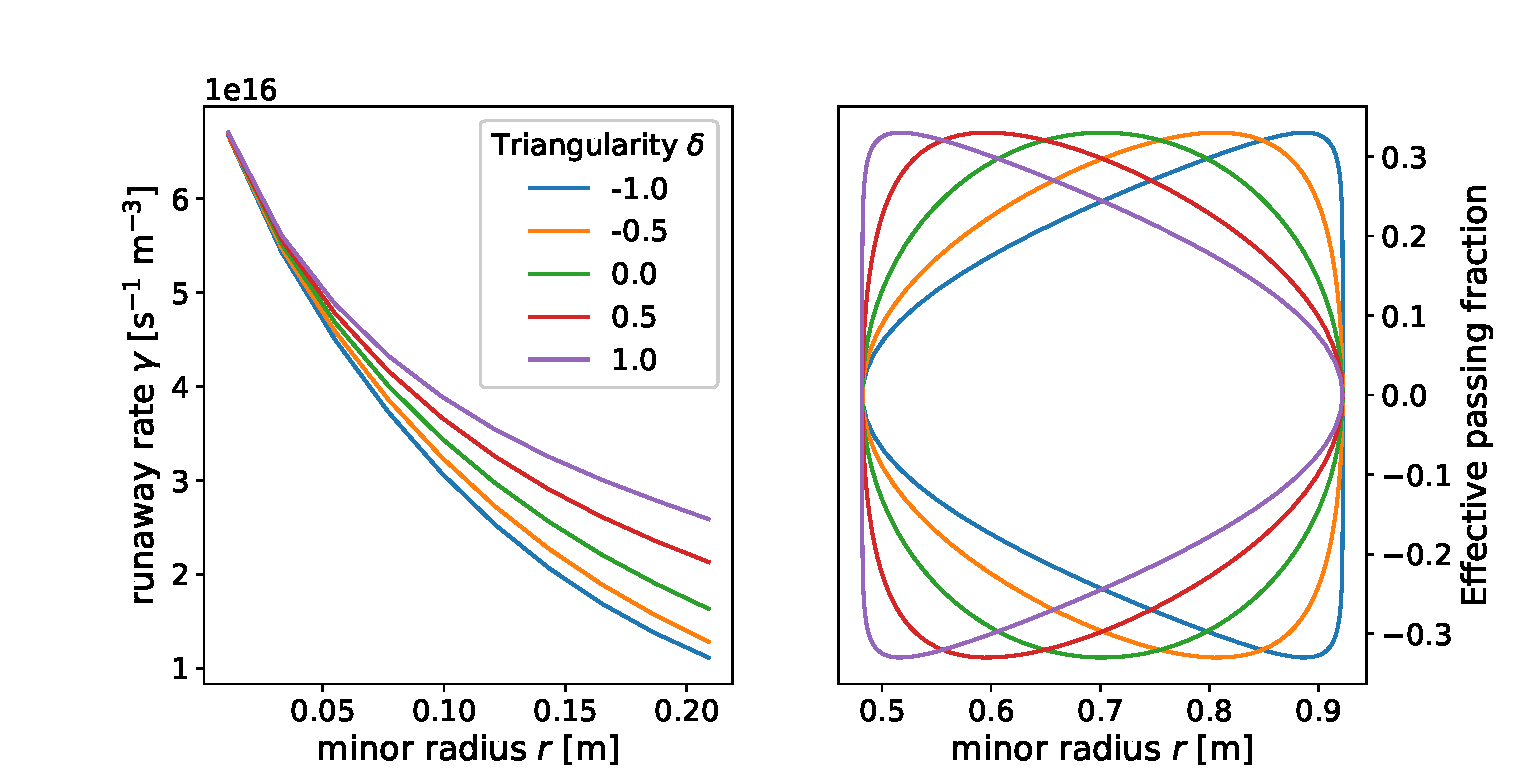
\includegraphics[width=\textwidth]{figs/triangularity.eps}
    \caption{\textit{Flux surface averaged electron runaway rate $\langle\diff{n}_{re}/\diff{t}\rangle$ vs.\ minor radius coordinate $r$ for fice different triangularity $\delta$ (left), and corresponding tokamak cross sections (right).}}
    \label{fig:elongation}
\end{figure}

\subsection{Dependence on Shafranov shift}
\begin{figure}[H]
    \centering
    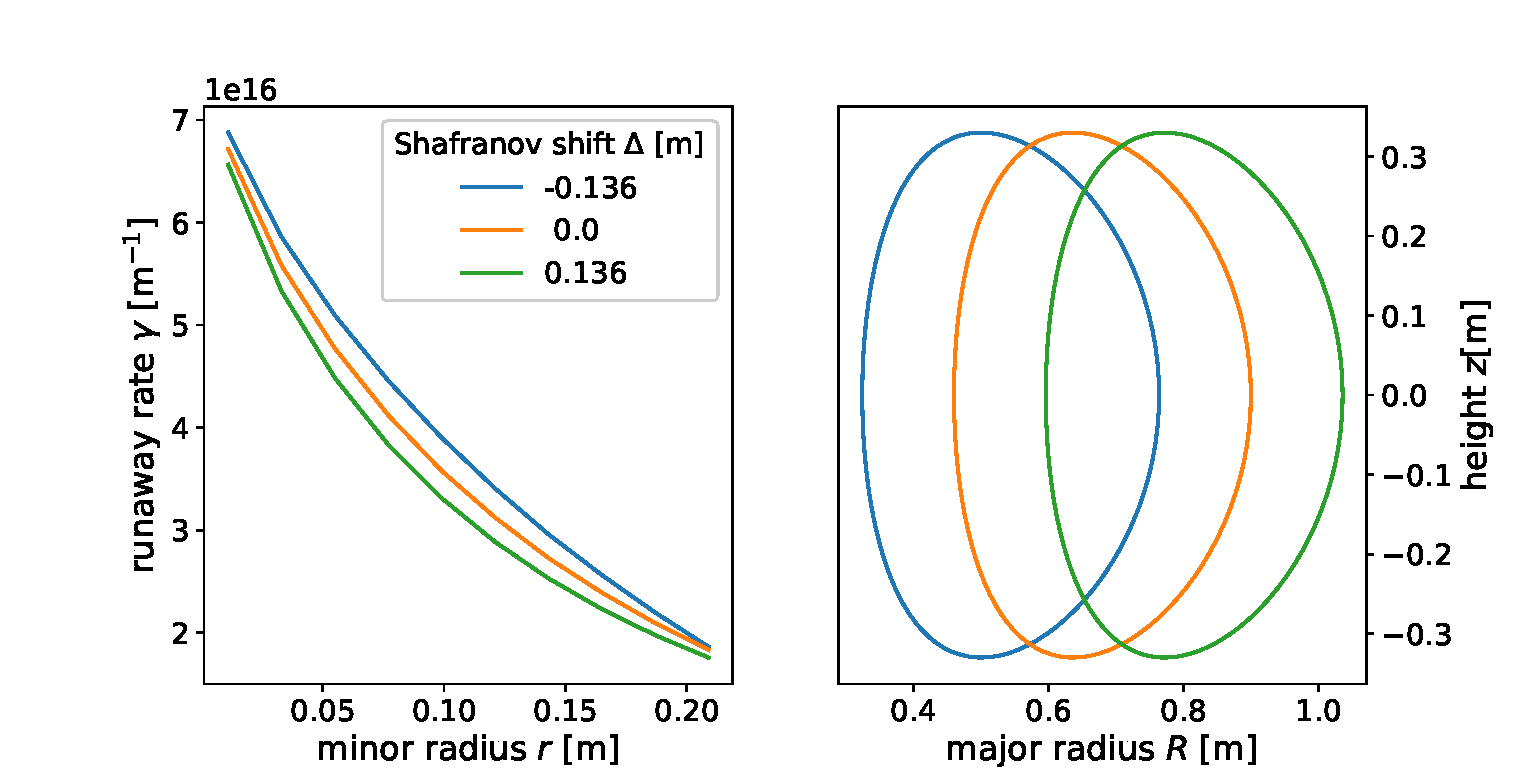
\includegraphics[width=\textwidth]{figs/shafranovShift.eps}
    \caption{\textit{Flux surface averaged electron runaway rate $\langle\diff{n}_{re}/\diff{t}\rangle$ vs.\ minor radius coordinate $r$ for three different Shafranov shifts $\Delta$ (left), and corresponding tokamak cross sections (right).}}
    \label{fig:shafranovShift}
\end{figure}

\begin{thebibliography}{100}
    \bibitem{DREAM}
    DREAM documentation, \url{https://ft.nephy.chalmers.se/dream/index.html} (accessed 21/9/21)

\end{thebibliography}




\end{document}
